\chapter{Ambiente di Lavoro}

Per far funzionare \LaTeX{} sul vostro computer dovete scaricare un
compilatore, che potete trovare a questo all'indirizzo
\url{https://miktex.org/download}. L'installazione è facile ma il completamento
potrebbe richiedere un po' di tempo. Siate pazienti.
Per gli scopi di questo corso utilizzeremo \textbf{TeXnicCenter}, un comodo IDE
che potete scaricare gratuitamente all'indirizzo
\url{http://www.texniccenter.org/download/}.
Ovviamente avrete bisogno anche di un visualizzatore PDF, in questo caso noi
consigliamo un lettore PDF leggero e veloce (cosa che Adobe Reader non è), che
ci sarà molto utile in quanto dovremo aprirlo ripetutamente: il lettore PDF in
questione si chiama SumatraPDF ed è gratuitamente scaricabile al seguente
indirizzo \url{https://www.sumatrapdfreader.org/download-free-pdf-viewer.html}.
In ogni caso siete liberi di utilizzare il lettore PDF che più preferite.

\section{Windows e TeXnicCenter}

Durante la prefazione (che nessuno di voi avrà certamente letto) abbiamo
parlato di IDE. Per il nostro corso ne utilizzeremo uno (come già detto sopra)
e in questo capitolo vedremo un attimo alcune delle sue funzionalità, giusto
per prendere mano con l'ambiente che dovremo usare.

Se avete installato TeXnicCenter sul vostro computer per la prima volta e lo
state aprendo solo ora vi chiederà alcune informazioni riguardo al lettore DVI
e PDF da usare. Riguardo al lettore DVI potete pure lasciare i campi vuoti,
mentre per il lettore PDF premete i tre puntini accanto alla prima casella di
testo, e selezionate nel vostro hard disk l'eseguibile del lettore PDF che più
preferite.

Prima di tutto, alla apertura del programma ci troveremo ad una schermata
vuota, in cui possiamo vedere diversi bottoni.

\begin{figure}[H]
  \centering
  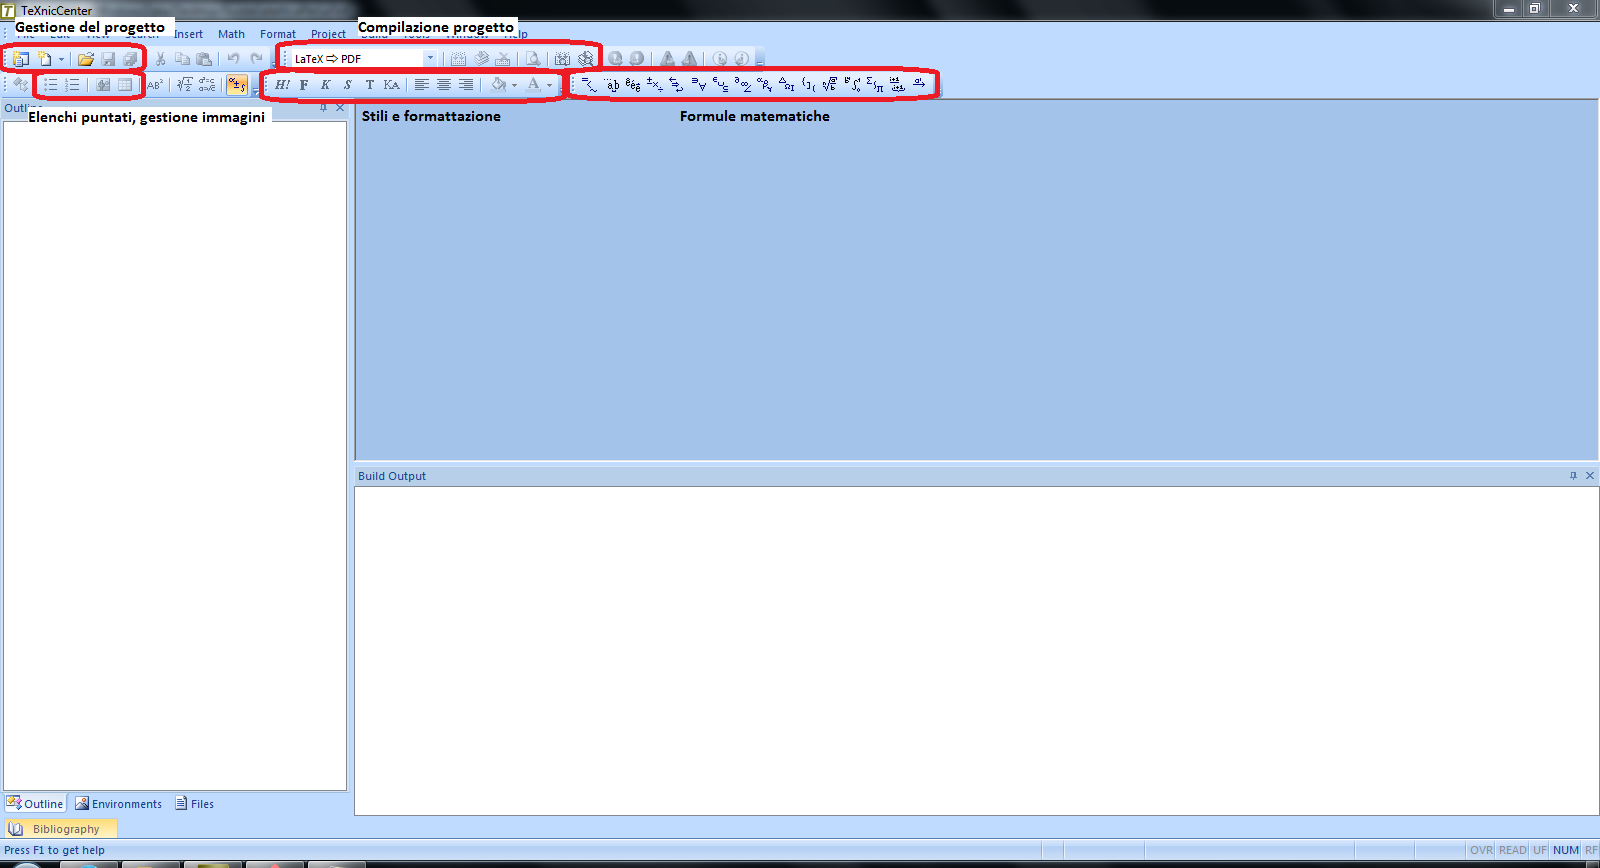
\includegraphics[scale=0.35]{texniccenterprincipale}
  \caption{Schermata principale di TeXnicCenter}
  \label{img:principale_texcenter}
\end{figure}

\begin{figure}[H]
 \centering
 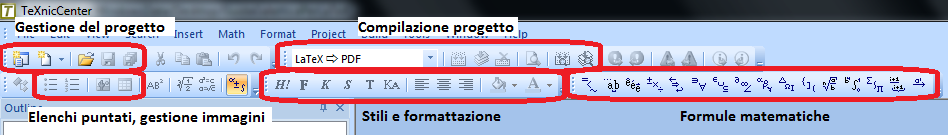
\includegraphics[scale=0.6]{texniccenterzoom}
 \caption{Zoom della schermata principale di TeXnicCenter}
 \label{img:principale_texcenter2}
\end{figure}


Come possiamo vedere dall'immagine\footnote{Sappiamo che si vede poco
ma questo è il meglio che siamo riusciti a fare} notiamo partendo da in alto
a sinistra e scorrendo verso destra che inizialmente troviamo dei bottoni per
gestire il progetto (o per crearne di nuovi).
Abbiamo subito dopo le opzioni per la compilazione: il menù a tendina ci
permette di selezionare che tipo di output vogliamo (se PDF o altri formati) e
i bottoni accanto a questo menù ci permettono di lanciare la compilazione
del progetto.
Nella seconda riga troviamo le impostazioni per la creazione di elenchi puntati
e numerati senza necessità di scrivere codice, seguiti dai bottoni per
aggiungere immagini e tabelle. Nel penultimo riquadro ci sono i classici bottoni
per impostare gli stili di formattazione (quelli che siamo abituati ad avere in
Word per intenderci).
Alla fine troviamo i bottoni per l'inserimento di formule matematiche, che
tratteremo più avanti in questa guida.

\subsection{Creare un progetto}

Iniziamo ora la creazione di un progetto.
Clicchiamo su \texttt{New Project} e selezioniamo il modello vuoto. Spuntiamo
la casellina \texttt{Uses BibTeX} nella sezione \texttt{Features}, e diamo un
nome al nostro progetto. Fatto ciò il bottone \texttt{Ok} dovrebbe essersi
sbloccato, e lo clicchiamo. Il programma creerà le basi necessarie per
cominciare un nuovo progetto!\footnote{Nota, se volete potete selezionare il
percorso che preferite dove salvare il progetto.}
Il progetto che avremo davanti è però vuoto, e consisterà di un unico file: per
progetti \LaTeX{} grandi è generalmente buona pratica separare quelle che sono
le impostazioni del progetto (come configurazione dei pacchetti e importazione
degli stessi) dal contenuto (ovvero quello che è il vero e proprio documento).
Questo permette poi di eseguire modifiche più facilmente, e di avere un maggior
ordine nel progetto stesso.
La struttura consigliata potrebbe essere\footnote{Consigliata in quanto non ne
esiste una unica, questa è quella che negli anni gli autori si sono trovati
meglio ad utilizzare.}:
\begin{verbatim}
 <nomeprogetto>.tex
 res/
 -- config/
 ---- config.tex
 ---- package.tex
 -- sections/
 -- img/
 listOfSections.tex
\end{verbatim}

Spiegheremo brevemente perché:
\begin{itemize}
  \item Il \texttt{<nomeprogetto>.tex} è buona pratica che contenga solo il
codice necessario per importare i vari pezzi del progetto, e per darne le
informazioni di base
  \item In \texttt{res/} ci saranno le risorse vere e proprie del progetto, che
sono composte dai file di configurazione, dalle varie immagini e da altri file
TeX, che possono rappresentare capitoli o parti (la suddivisione è a proprio
piacimento)
  \begin{itemize}
   \item Abbiamo il file \texttt{config/} dove configurare i vari pacchetti
(per esempio scriviamo lì se preferiamo avere i link di colore rosso al posto
di blu), mentre nell'altro file, \texttt{package.tex}, abbiamo tutte le
importazioni necessarie per far compilare il documento. In questa maniera, se
un pacchetto dovesse a detta del compilatore risultare mancante potremmo subito
controllare se avrà ragione o meno\footnote{E l'avrà perché i computer sono
macchine, e le macchine se programmate bene hanno la tendenza e non sbagliare.}
  \item In \texttt{img} metteremo tutte le immagini, così da avere un unico
posto dove salvarle e eviteremo in questa maniera di spargerle su tutto il
progetto.
  \item \texttt{listOfSections} grazie alla \textit{keyword} \verb!\include{ }!
possiamo includere diversi file, ed è consigliato includere qui la lista delle
sezioni/parti che vogliamo vengano compilate nel documento.
  \end{itemize}
\end{itemize}

Il funzionamento e l'inclusione dei file in \LaTeX{} è un argomento importante
che verrà meglio spiegato in \ref{sec:prog_piu_file}.

Ora che abbiamo un progetto vuoto possiamo praticamente fare quello che
vogliamo! Siccome è la prima volta, proviamo a fare un progetto che ci stampi
due pagine, uno con il titolo e l'altra con una scritta e una figura.

\subsubsection{Hello world!}

In Informatica è buona pratica iniziare sempre con un programmino semplice che
stampi una scritta di saluto. Noi ovviamente non ci sottrarremo dalla
tradizione, per cui faremo lo stesso.

\paragraph*{File principale} Dal nostro progetto vuoto inseriamo il seguente
codice nell'unico file che abbiamo:

\lstinputlisting{res/examples/Prova/Prova.tex}

\noindent Cosa stiamo dicendo qui? Stiamo dicendo prima di tutto che vogliamo
includere il file contenente la lista dei pacchetti (che dobbiamo ancora
scrivere) e che vogliamo includere il file con le configurazioni dei pacchetti
che abbiamo incluso prima. Dopo abbiamo settato l'autore, la data, e il titolo
del nostro documento.
Finito il preambolo abbiamo iniziato con il contenuto, in cui abbiamo detto a
\LaTeX{} di creare una pagina standard di copertina, e poi gli diciamo di
andare ad includere anche i contenuti che sono presenti nel file
\texttt{listOfSections} che si trova nella sottocartella che andremo a creare
\texttt{res/}.

\paragraph*{File \texttt{res/config/package.tex}} Dalla interfaccia di
\texttt{TeXnicCenter} andiamo a cliccare il bottone per creare un nuovo file
(che è accanto a quello per creare un nuovo progetto, in alto a sinistra). Si
aprirà una scheda con un nuovo file vuoto. Qui scriviamo:

\lstinputlisting{res/examples/Prova/res/config/package.tex}

\noindent Qui gli stiamo specificando come vogliamo creare un documento che
sarà un libro, di usare il carattere 12 quando non specificato e di includere
due pacchetti: \texttt{graphicx} e \texttt{float}.
Quando andiamo a salvare ora andiamo nel nostro progetto e creiamo due nuove
cartelle, \texttt{res} e dentro questa cartella creiamo \texttt{config}.
All'interno di quest'ultima salviamo il nostro file, impostando la voce
\texttt{Encoding} in \texttt{UTF-8}\footnote{Questo ci serve per aggiungere
compatibilità con gli accenti}.

Ora passiamo al file successivo.

\paragraph*{File \texttt{res/config/config.tex}} Andiamo a creare questo file
come al solito. In questo progetto non abbiamo nessuna configurazione
particolare, e quindi lo possiamo lasciare vuoto. In caso dovessimo inserire
qualche configurazione potremmo modificarlo più avanti.

\paragraph*{File \texttt{res/listOfSections.tex}} Creiamo questo file con il
seguente contenuto:

\lstinputlisting{res/examples/Prova/res/listOfSections.tex}

\noindent Anche in questo caso, facciamo attenzione alla voce \texttt{Encoding}
quando andiamo a salvarlo. Questo file conterrà solamente inclusioni ai veri
contenuti di testo, permettendoci di escludere parti o riordinarle senza fare
fastidiosi copia-incolla.

Passiamo ora al file nel quale mettere veramente il nostro contenuto.

\paragraph*{File \texttt{res/sections/parte1.tex}} Per prima cosa, con Esplora
Risorse prendiamo l'immagine che più ci piace e copiamola in \texttt{res/img/}
(creando la cartella \texttt{img}). Creando un nuovo file, ora inseriamo questo
codice:

\lstinputlisting{res/examples/Prova/res/sections/parte1.tex}

\noindent Cosa abbiamo qui? Prima di tutto, abbiamo una normale scritta, che
contiene il nostro famoso saluto. Proviamo ora a includere l'immagine.
Ci sono due modi per farlo:
\begin{itemize}
 \item Scrivere direttamente il codice (scelta consigliata)
 \item Includere l'immagine tramite TeXnicCenter
\end{itemize}

Nel primo caso, dobbiamo solo copiare il codice, mentre nel secondo caso
andiamo a cliccare l'icona a forma di immagine che si trova in alto a sinistra
(per chi non trovasse l'icona veda l'immagine \ref{img:principale_texcenter},
nel quadrato con l'etichetta \textit{Elenchi puntati, gestione immagini}).
A questo punto si aprirà una finestrella che ci chiederà di inserire il
percorso dell'immagine e altre opzioni. Fatto ciò andiamo a selezionarla
premendo sul bottone con i tre puntini.

\begin{figure}[H]
 \centering
 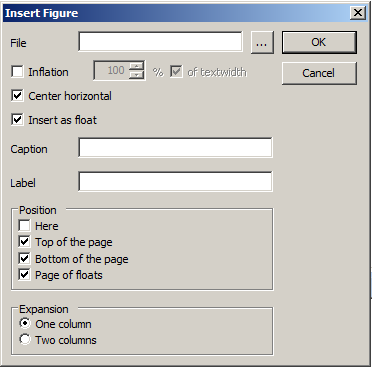
\includegraphics[scale=0.6]{insert_figure}
 \caption{Finestra per l'inserimento di una nuova immagine nel documento}
 \label{img:insert_figure}
\end{figure}

Selezioniamo anche la spunta ``Here'' e inseriamo una \textit{caption} e una
\textit{label} che più ci aggradano (non inserite caratteri speciali nella
\textit{label} o il documento non compilerà più).

\paragraph*{Compilazione} Prima di compilare settiamo l'output di compilazione.
Nel menù a tendina selezioniamo la voce ``LaTeX $\to$ PDF''. Ora clicchiamo il
quinto bottone a partire dal menù (muovendoci da sinistra verso destra). Se
abbiamo seguito le istruzioni correttamente, si aprirà il visualizzatore PDF
con quanto abbiamo scritto. Complimenti! Avete creato il vostro primo PDF
usando \LaTeX{}.

\begin{figure}[t]
 \centering
 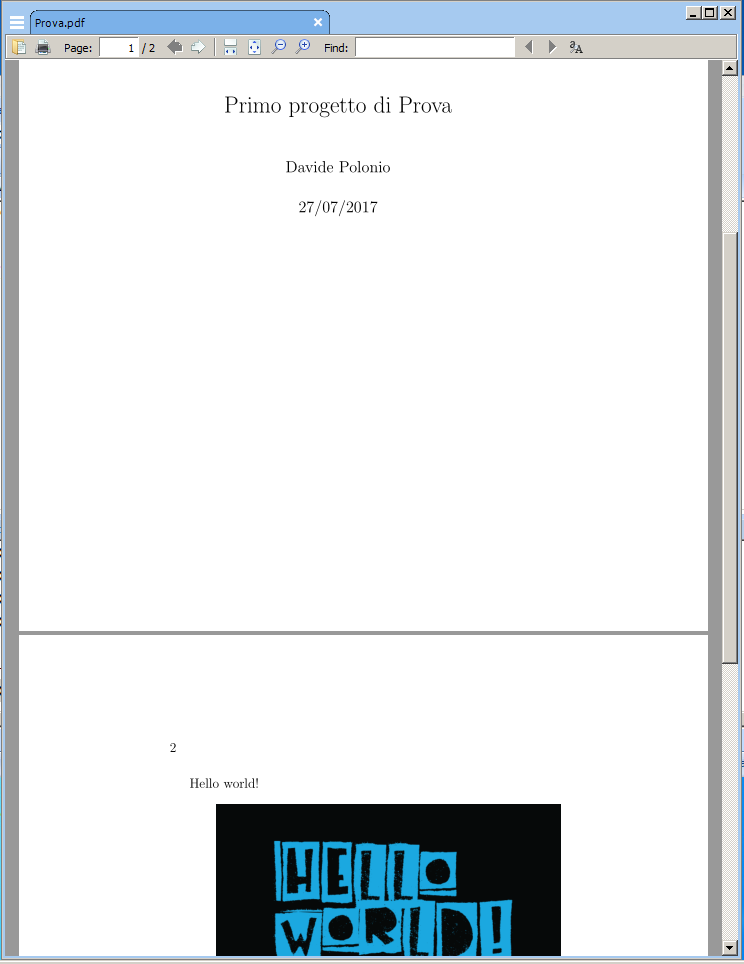
\includegraphics[scale=0.5]{compilation_res}
 \caption{Il risultato che dovremmo ottenere}
 \label{img:compilation_res}
\end{figure}

\paragraph*{Dove trovare il progetto} Se volete vedere il documento di prova
che abbiamo fatto fino ad adesso (e per dimostrarvi che non vi abbiamo
trollato ma che l'abbiamo fatto anche noi e che funziona) potete recarvi alla
seguente pagina web e guardare i singoli file
\url{
https://github.com/R-and-LaTeX/GuidaGalatticaPerLaTeX/tree/develop/res/examples/
Prova}.

\newpage

\section{Compilare su Linux/MacOS}

La compilazione di un progetto su Linux/MacOS risulta più semplice e
fortunatamente più facile da spiegare. In generale, dopo aver installato tutte
le dipendenze necessarie per l'ambiente \LaTeX{}, basta solitamente aprire un
terminale nella \texttt{root} del progetto e dare il comando magico
\texttt{latexmk -pdf} che si occuperà di compilare il tutto il numero giusto di
volte.

\section{Suddivisione del progetto in più file}
\label{sec:prog_piu_file}

Come abbiamo visto prima, anche un semplice progetto come un \textit{Hello
World} può risultare nella creazione di 4-5 file. Non preoccupatevi! È un
fenomeno normale in \LaTeX{}.
Per includere diversi file in \LaTeX{} esistono due comandi:
\begin{itemize}
 \item \verb!\input{ }! questo comando concatena i documenti considerandoli
come se fosse uno unico, e permette di concatenare file fino a qualsiasi
profondità.
 \item \verb!\include{ }! la seguente \textit{keyword} inserisce della magia,
come un'interruzione di pagina e crea altri file utili a tempi di
compilazione. Questo comando è solitamente utile quando si ha un progetto
grande su computer molto lento, in quanto il cambiamento di un file non
comporta la ricompilazione completa di tutto il documento, anche se non
supporta inclusioni annidate (chiamare \verb!\include{ }! su un altro file che
è già stato incluso con \verb!\include{ }! produrrà un errore). Per quello che
ci serve a noi, è meglio usare sempre il primo comando.
\end{itemize}

\paragraph*{Suddivisione del contenuto in \texttt{res/sections/}} In generale,
non c'è una regola predefinita per suddividere il proprio contenuto: questo può
essere suddiviso per capitoli se per esempio si sta scrivendo una tesi, oppure
per sezioni se invece si sta scrivendo una pubblicazione scientifica, il tutto
dipende dalla granularità che si vuole dare al documento, e alla facilità con
cui si vogliono spostare gli argomenti.
